    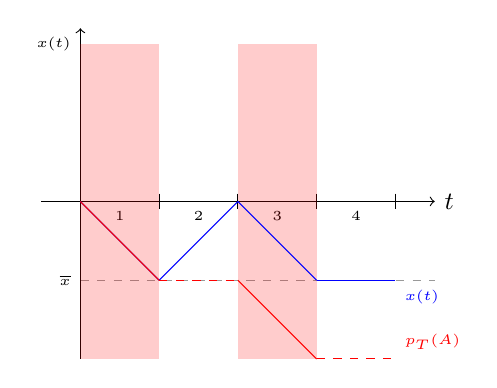
\begin{tikzpicture}
        % Draw x-axis

        \draw[->] (-.5,0) -- (4.5,0) node[right, font=\small] {$t$};
        \draw[dashed, opacity=0.4] (0,-1) -- (4.5,-1);
        \node at (0, -1) [left, font=\tiny] {$\overline{x}$};
        % Draw y-axis
        \draw[->] (0,-2) -- (0,2.2);

        \node at (0, 2) [left, font=\tiny] {$x(t)$};

        % Add ticks on x-axis
        \foreach \x in {1,2,3,4}
            \draw (\x,0.1) -- (\x,-0.1);
        
        \foreach \x in {1,2,3,4}
            \draw (\x - 0.5 ,0) -- (\x-0.5,-0) node[below, font=\tiny] {\x};

        % Shade a vertical region
        \foreach \x in {1, 3}
            \fill[red, opacity=0.2] (\x-1,-2) rectangle (\x,2);
        \draw[-, blue] (0, 0) -- (1, -1);\draw[-, blue] (1, -1) -- (2, 0);\draw[-, blue] (2, 0) -- (3, -1);\draw[-, blue] (3, -1) -- (4, -1);\node at(4, -1) [below right, blue, font=\tiny] {$x(t)$};
        \draw[red, -] (0, 0) -- (1, -1);\draw[red, dashed] (1, -1) -- (2, -1);\draw[red, -] (2, -1) -- (3, -2);\draw[red, dashed] (3, -2) -- (4, -2);\node at (4, -2) [above right, red, font=\tiny] {$p_T(A)$};
            
    \end{tikzpicture}

    